\chapter{\uppercase{Conclusions, Future Work, and Preliminary Results} \label{chapter:future}}


\section{Concluding Remarks}
In the Chapter~\ref{chapter:mud} we demonstrate that the MUD solution retains the accuracy of least-squares solutions while simultaneously offering the flexibility of specifying initial beliefs.
Normally in order to incorporate such beliefs, practitioners in the machine-learning field would perform Tikhonov regularization, usually with the inclusion of a hyper-parameter which scales the additional parameter-space norm in the objective function.
Mathematically, this scaling factor applied to the norm is equivalent to scaling the matrix representation of an initial (prior) covariance and searching for the MAP point of a Bayesian posterior.
Increasing this scaling factor is interpreted as having less confidence in these initial assumptions.
Conversely, decreasing it is equivalent to putting more emphasis on the prior beliefs than the evidence provided by the data, which causes MAP solutions to drift away from the solution contour (equivalence class) to which $\paramref$ belongs.

The MUD point is not impacted by scaling of the initial covariance, providing \emph{consistent} solutions which demonstrate levels of accuracy that MAP points only exhibit for larger values of scaling factors.
Not only is it robust to the specification of prior assumptions, but it manages to offer the flexibility of such specifications without paying the additional cost of hyper-parameter optimization that would be required for the Tikhonov solution to achieve comparable results; any choice of $\alpha$ would have sufficed.

By contrast, the Tikhonov-regularized solution selects a point that is biased in directions defined by the initial density (covariance).
The data-consistent solution is an update to the initial mean in this same direction but will always exist on the contour $Q^{-1}(\observedMean)$, where $\observedMean$ is the mean of the observed density.


We also show that regardless of how well-informed the initial beliefs are, the convergence rate of the MUD solutions as more data are incorporated\---either by dimension or rank)\---will match those of the Least-Squares solutions.
Moreover, unlike MAP solutions, the MUD point is not sensitive to scaling of the initial covariance (how strongly initial beliefs are held).
This insensitivity provides a strong motivating factor for the consideration of the data-consistent approach within the standard set of solution methods available to scientists and modelers who seek to perform parameter-identification.
We leave the investigation of more connections to the removal of hyper-parameter estimation to future work.

The trouble is, none of these regularization approaches actually guarantee that in under-determined problems, the unique solutions that are selected are close to $\paramref$.
The equivalence-class nature of the solution contour means that by definition there are directions in which uncertainty is unresolved.
Thus, the goal is to aggregate data into components of a vector-valued QoI map to improve estimates of $\paramref$ across more dimensions.
We use skewness as a guide for constructing the QoI and demonstrate its utility in improving estimates to a $\paramref$ related to estimating an uncertain function.


\section{Future Work and Preliminary Results}

\subsection{Optimal Experimental Design Considerations}

In this section we return to the nonlinear examples presented in the previous chapter and address some choices made in how the experiment was performed.
By revisiting the examples, we demonstrate that the decisions made regarding measurement equipment and/or location have an impact on the reduction of uncertainty and accuracy of the MUD point.
Furthermore, we want to show that the choices made in the experimental design of previous examples were made for reasons of convenience of exposition.
Changing these assumptions does not later the viability of the MUD point as an alternative estimator for use parameter identification problems.
We study the impact of more precise measurement devices on the convergence rates for the parameter estimates in Appendix \ref{ext:ode-example} for the problem in \ref{subsec:ode-example} of estimating the rate of exponential decay.
To complement these results, we show them alongside ones generated with equipment that measures at twice the temporal frequency.

We highlight how an awareness of another geometric property of QoI maps---relating to their sensitivity with respect to $\param$---can help improve the accuracy of the MUD estimate.
By placing sensors in locations which exhibit greater sensitivity to the parameter for which the SIP is solved, experimenters can achieve a considerable improvement in the precision of estimating $\paramref$ with an equal number of measurements collected.
A similar complementary problem is solved where information about the sensitivity of measurement locations is used to inform improved placement of a hundred sensors.
In this example, we walk through the sorts of analyses a modeler might conduct in order to select an experimental design through simulation and show a significant improvement in the accuracy of the MUD point.


%%%%%%%%%%%%%%%%%%%%%%%%%%%%%%%%%%%%%%%%%%%%%%%%%%%%%%%%%%%%%%%%%%%%
%%%%%%%%%%%%%%%%%%%%%%%%%%%%%%%%%%%%%%%%%%%%%%%%%%%%%%%%%%%%%%%%%%%%
\FloatBarrier
%%%%%%%%%%%%%%%%%%%%%%%%%%%%%%%%%%%%%%%%%%%%%%%%%%%%%%%%%%%%%%%%%%%%
%%%%%%%%%%%%%%%%%%%%%%%%%%%%%%%%%%%%%%%%%%%%%%%%%%%%%%%%%%%%%%%%%%%%
\subsection{Elliptic PDE Example}\label{sec:pde-example}
We make a slight modification to the Poisson problem from \ref{subsec:pde-example} to make it into a one-dimensional parameter identification problem.
This choice is primarily motivated by the goal of using visual aids to demonstrate slopes corresponding to different measurement locations.
We briefly summarize the experimental set-up again for the reader's convenience
Consider the following Poisson problem defined on a unit domain $\Omega$:
\begin{equation}\label{eq:pde-equation}
\begin{cases}
\hfill -\nabla \cdot \nabla u &= f \quad\text{on } \Omega \\
\hfill u &= 0 \quad\text{ on } \Gamma_T \cup \Gamma_B \\
\hfill \frac{\partial u}{\partial \mathbf{n}} &= g(x,\param) \quad\text{ on } \Gamma_L \\
\hfill \frac{\partial u}{\partial \mathbf{n}} &= 0 \quad\text{ on } \Gamma_R
\end{cases}
\end{equation}
where $(x_1, x_2) \in \Omega = (0,1)^2$, $\Gamma_T$ is the top, $\Gamma_B$ is the bottom, $\Gamma_L$ and $\Gamma_R$ left and right, respectively.
$\frac{\partial u}{\partial \mathbf{n}}$ denotes the outward normal direction.
We select $g=\param \sin(\pi x_2)$, and show the response surface for our given choice of $\param = 3$ in the left of Figure~\ref{fig:pde-response}, with darker colors representing more negative values.
Our initial density is chosen to be uniform over the interval $\Lambda = (1,5)$.
$f$ is chosen to be $10\exp\{-\frac{(x_1-0.5)^2 + (x_2 - 0.5)^2}{0.02}\}$


We are interested in demonstrating the impact of incorporating more measurements on our ability to estimate $\paramref$.
%This poses a problem for this particular experimental design since it will heavily rely on the way in which the sensor grid is indexed.
%One could place a regular grid of sensors in the interior of $\Omega$ to simulate a structured sensor array.
%However, observe that the response surface shown on the left panel of Figure~\ref{fig:pde-response} exhibit vertical symmetry about the line $x_2=0.5$ (as a result of our choice of $g$).
%For example, if the first half of indexed sensors corresponded to the bottom half of $\Omega$, the incorporation of the second half will be equivalent to having repeated observations.
%To avoid these problems, we instead simulate the sensors as being placed randomly (drawn from uniform distributions), in the interior so that index-dependence becomes irrelevant and probability theory ensures the lack of truly redundant measurement locations.
In \cite{Walsh}, the geometric quantity known as \emph{scaling} inherent to QoI maps is studied with respect to its impact on the accuracy of solutions to SIPs.
This property corresponds to the average local linear response of the QoI map with respect to changes in $\param$.
In short, if a QoI map (such as one induced by a single measurement), exhibits larger slopes on average over $\pspace$, then it has greater scaling and by implication, more predictive precision.
We demonstrate how an awareness of the QoI's scaling can inform the construction of a more optimal QoI map by way of better selecting the locations of measurement devices.
Here, the assessment of a map's average scaling is identified heuristically through visual inspection of slopes.
Such a graphical comparison of QoI maps can be done without prior knowledge of the scaling property and is not outside the scope of analysis that could be performed during initial investigation into an inverse problem.

%%%%%%%%%%%%%%%%%%%%%%%%%%%%%%%%%%%%%%%%%%%%%%%%%%%%%%%%%%%%%%%%%%%%
\FloatBarrier
%%%%%%%%%%%%%%%%%%%%%%%%%%%%%%%%%%%%%%%%%%%%%%%%%%%%%%%%%%%%%%%%%%%%
\subsubsection{Uninformed Sensor Placement}
First we show that using the sensor-placement strategy introduced in \ref{subsec:pde-example} results in many locations that provide little information to reduce uncertainty in the parameter space.
We consider a selection of $S=1000$ measurement locations in the interior of the response surface chosen by sampling a uniform density over the set $(0.05, 0.95)^2 \subset \Omega$.
We show only the first hundred measurement locations in plots for visual clarity.
In the rightmost histogram of Figure~\ref{fig:pde-response}, we plot the data generated by each simulated sensor location, and note that many values are near zero as a result of being near boundaries or the right-side of $\Omega$.

\begin{figure}
\centering
  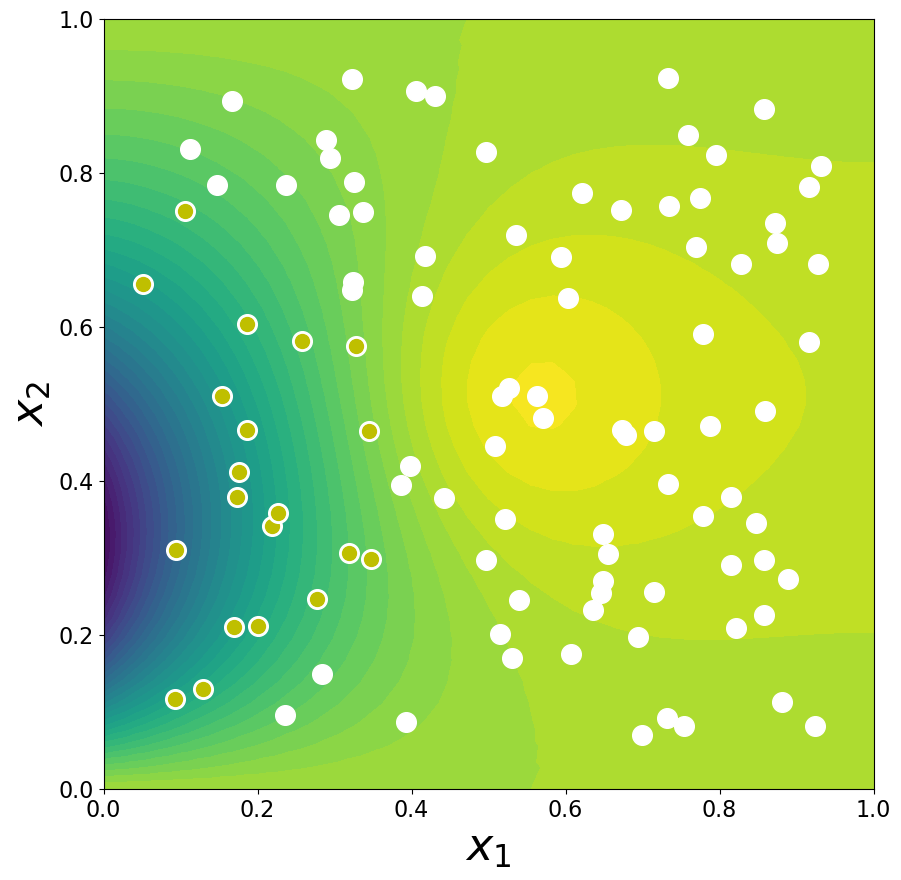
\includegraphics[width=0.25\linewidth]{figures/pde/pde_reference_solution}
  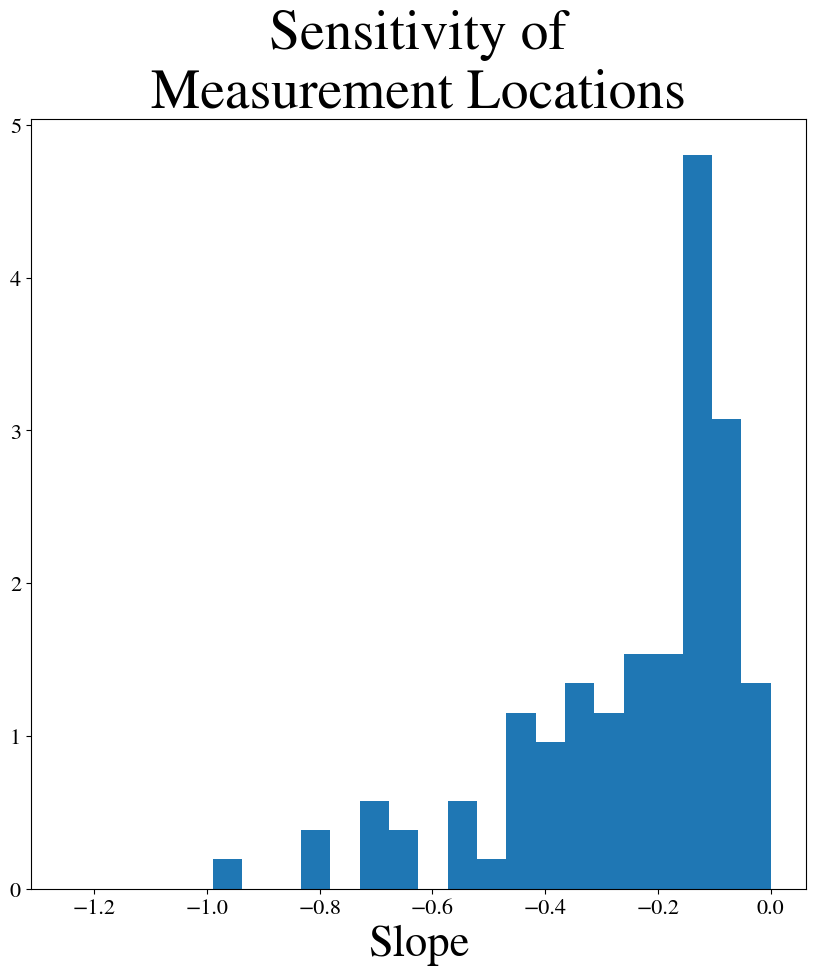
\includegraphics[width=0.25\linewidth]{figures/pde/pde_sensitivity_qoi}
  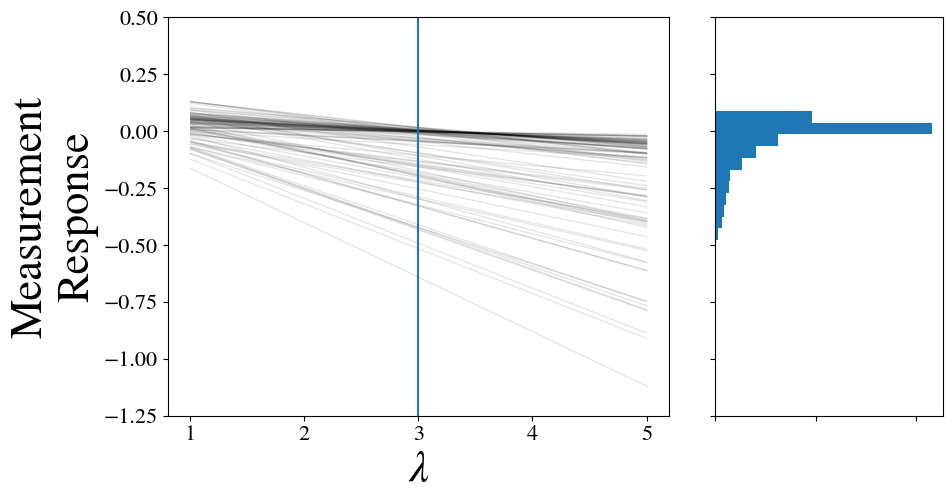
\includegraphics[width=0.45\linewidth]{figures/pde/pde_qoi_response}
\caption{(Left): The function response surface for $u$ solving \eqref{eq:pde-equation} with $S=100$ measurement locations highlighted in white.
The twenty most sensitive location markers are filled.
(Right): The derivative $\partial M_i / \partial \param$ is computed for the hundred measurement locations and the distribution of the resulting collection of slopes is plotted.
(Center): The values of the response surface at the hundred measurements is shown. The true parameter value $\paramref$ is highlighted with a vertical line, and the values of the response surface conditioned on $\paramref$ are used to form the histogram plotted vertically on the right. Many measurements are near zero.
}
\label{fig:pde-response}
\end{figure}

The measurement response as a function of $\param$ is plotted next to it in the center of \ref{fig:pde-response}, and suggests that the sensors each exhibit linear responses to changes in the parameter.
This observation can be used to visually identify that some measurements are more sensitive than others since the lines from certain sensors have steeper slopes than the majority of locations.
The majority of measurements exhibit almost no sensitivity to changes in $\param$, visually represented by the density of nearly horizontal lines (slopes of zero).
However, some of the sensors have steep slopes, which suggests higher sensitivity to changes in $\param$.
To quantify the variability in the slopes across different sensor locations, we use the smallest and largest samples values of $(\param, u(\param))$ to make a global linear estimate of each one's slope.
We plot the distribution associated with the collection of these slopes in the center histogram of \ref{fig:pde-response}.
%%%%%%%%%%%%%%%%%%%%%%%%%%%%%%%%%%%%%%%%%%%%%%%%%%%%%%%%%%%%%%%%%%%%
% \vfill
\FloatBarrier
%%%%%%%%%%%%%%%%%%%%%%%%%%%%%%%%%%%%%%%%%%%%%%%%%%%%%%%%%%%%%%%%%%%%
\subsubsection{Informed Sensor Placement}
Instead of placing sensors throughout the square interior of $\Omega$ given by $(0.05, 0.95)^2$, we consider how the convergence results would compare if the subdomain for sensors was better selected.
In the left panel of Figure~\ref{fig:pde-response}, the most sensitive measurements are highlighted and appear near the left boundary.
Furthermore, the response surface exhibits horizontal symmetry, so we restrict locations to the bottom half of $\Omega$.
These two observations can inform a new bounding box for consideration of where measurements should be taken.
We perform the same experiment for sensors placed in $(0.05, 0.25)\times(0.05, 0.5)$ (measurement locations drawn from a uniform distribution over this region), and refer to this as the \emph{alternative} experimental design.
The first hundred of the thousand sensor locations sampled is shown in the left panel of \ref{fig:pde-alt-response} and we remark that the most sensitive ones (highlighted) cluster near the center of the left boundary, where the response surface is most negative.


\begin{figure}
\centering
  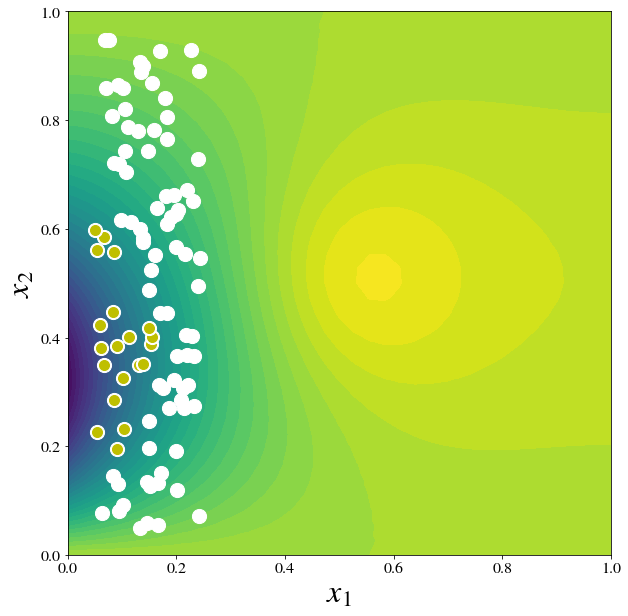
\includegraphics[width=0.25\linewidth]{figures/pde/pde-alt_reference_solution}
  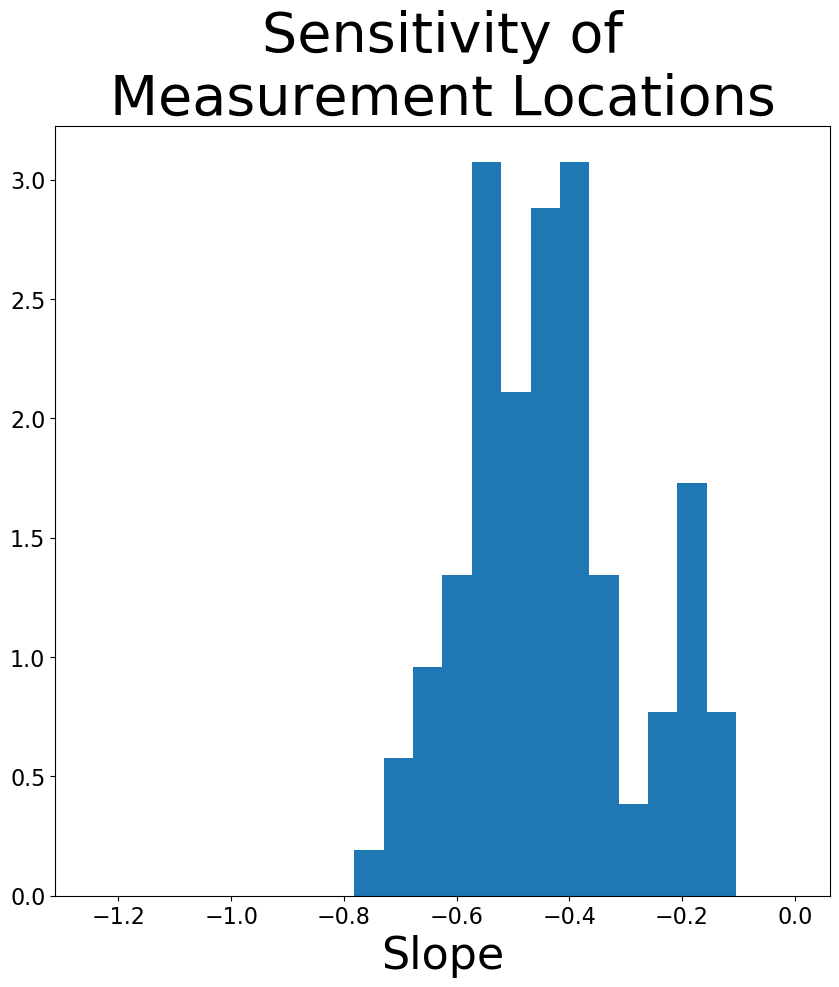
\includegraphics[width=0.25\linewidth]{figures/pde/pde-alt_sensitivity_qoi}
  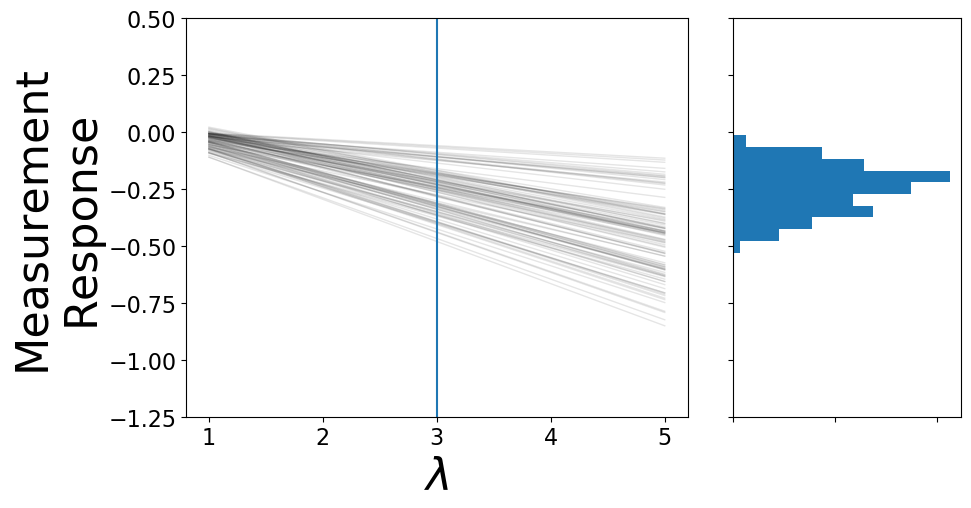
\includegraphics[width=0.45\linewidth]{figures/pde/pde-alt_qoi_response}
  \caption{The same panels as in Figure~\ref{fig:pde-response} but for the placement of sensors informed by the observations about sensitivity incorporated into the experimental design.
  The alternative placement eliminates redundancy induced by the symmetry of the response surface, and is concentrated in the regions which exhibit more sensitivity to changes in $\param$.
  As a result of these choices, we observe less measurements near zero (bottom histogram), and slopes with larger magnitude (top).
  }
\label{fig:pde-alt-response}
\end{figure}

For this alternative design, we show the sensitivity of sensors in the center of \ref{fig:pde-alt-response} and note that there are fewer sensors which exhibit low sensitivity to changes in $\paramref$ in contrast to \ref{fig:pde-response}.
The slopes are again shown in the center of the figure and exhibit a bimodal distribution with a larger portion of the measurements having slopes with magnitude 4-6 times greater than the mode in the center of \ref{fig:pde-response}.
There are also less measurements which take values near zero as well, shown in the rightmost panel of the figures.
The original design exhibited a strong decay in its distribution of measurement values, while the alternative design results in a much more symmetric distribution.

% \vfill
%%%%%%%%%%%%%%%%%%%%%%%%%%%%%%%%%%%%%%%%%%%%%%%%%%%%%%%%%%%%%%%%%%%%
\FloatBarrier
%%%%%%%%%%%%%%%%%%%%%%%%%%%%%%%%%%%%%%%%%%%%%%%%%%%%%%%%%%%%%%%%%%%%
\subsubsection{Comparison of SIP Solutions with Different QoI Maps}

We are interested in knowing how the uncertainty around the parameter estimate (the MUD point) changes as we incorporate more (noisy) data.
To generate convergence plots, we solve the problem repeatedly for $S = 5, 10, 15, 20, 25, 50, 100, 250, 500, \text{ and } 1000$ and take the mean and variance of the twenty trials for each value of $S$.
Consider the convergence plots in Figure~\ref{fig:pde-convergence-obs}, which demonstrates the impact of increasing $S$ on our ability to resolve $\paramref$.

\begin{figure}
  \centering
  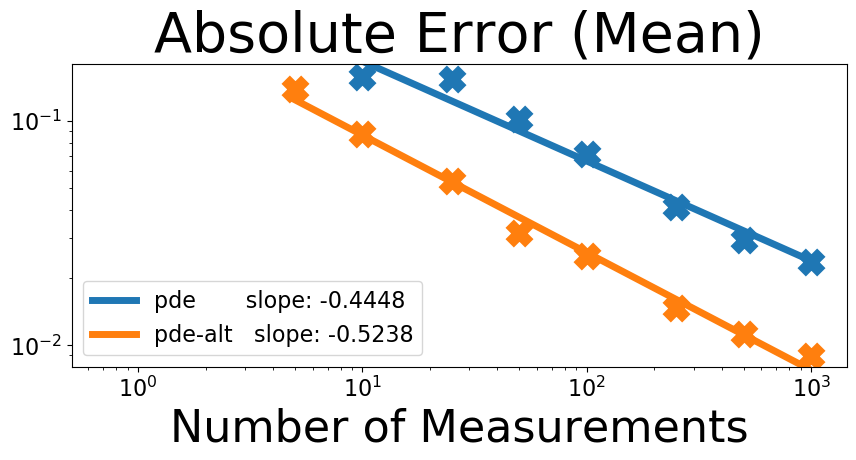
\includegraphics[width=0.475\linewidth]{figures/pde/pde_convergence_mud_obs_mean}
  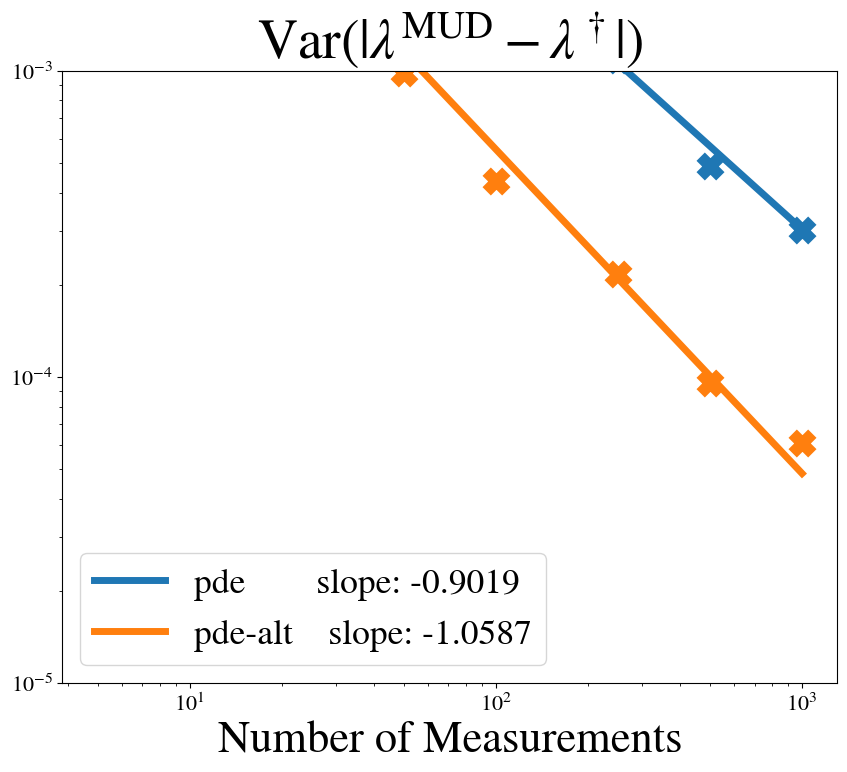
\includegraphics[width=0.475\linewidth]{figures/pde/pde_convergence_mud_obs_var}
  \caption{Convergence of the MUD point (given $N=1E3$ model evaluations) for increasing numbers of observations for randomly placed sensors.
  We observe similar rates of convergence for both arrangements of measurement locations, with a marked improvement in both accuracy and precision when an informed placement is used.
  }
  \label{fig:pde-convergence-obs}
\end{figure}

We show the mean absolute error in the left half of Figure~\ref{fig:pde-convergence-obs} and remark that two decimal places of accuracy can be achieved with approximately $250$ samples instead of the $1000$ required in the left-half.

In Appendix~\ref{ext:pde-tolerance}, we show these results for an experiment conducted with equipment of varying precision.

The convergence results for the original experimental design demonstrate that even randomly placed sensors in the interior of $\Omega$ are suitable for parameter estimation.
However, when we considered sensors that were placed with knowledge about the physical system being studied, more information was learned from our measurement equipment by placing sensors in different locations.
Using our alternative experimental design, we saw a reduction of uncertainty in both Figures~\ref{fig:pde-convergence-obs} and \ref{fig:pde-convergence-std}, represented by the persistent vertical displacement between the regression lines for convergence.


%%%%%%%%%%%%%%%%%%%%%%%%%%%%%%%%%%%%%%%%%%%%%%%%%%%%%%%%%%%%%%%%%%%%
%%%%%%%%%%%%%%%%%%%%%%%%%%%%%%%%%%%%%%%%%%%%%%%%%%%%%%%%%%%%%%%%%%%%
\FloatBarrier
%%%%%%%%%%%%%%%%%%%%%%%%%%%%%%%%%%%%%%%%%%%%%%%%%%%%%%%%%%%%%%%%%%%%
%%%%%%%%%%%%%%%%%%%%%%%%%%%%%%%%%%%%%%%%%%%%%%%%%%%%%%%%%%%%%%%%%%%%
%
% \subsection{Concluding Remarks}
% These examples demonstrate that Data--Consistent Inversion can be used for parameter identification as a viable alternative to existing methods.
% Incorporating available observations as we have done in the previous example leaves the output space scalar-valued.
% As the number of parameters grows, this output dimension resulting from such an approach effectively stays fixed.
% These situations are particularly when the DCI approach becomes advantageous over other methods, as it is less sensitive to mistakes in modeling assumptions than other methods for solving inverse problems as we saw with the linear examples in \ref{subsec:linear_examples} \ref{sec:high-dim-linear-example}.
% One can incorporate a much wider variety of prior beliefs about the relative likelihoods of parameters before data is collected without compromising predictive error.
% The DCI approach guarantees that the functional defined (for us, the weighted mean error) will remain accurate in spite of any encoded assumptions that are somehow at odds with data that is subsequently collected.

\FloatBarrier



%\subsection{Leveraging Data in Different Ways}\label{sec:ch05-data}
%Mention the other map we can use (SSE) here.
%
%\subsection{Addressing Model Assumptions}\label{sec:ch05-variance}
%Both the maps required us to have knowledge of the variance in the measurements.
%What if we got it wrong?
%\emph{What if we don't know the variance? How does mis-estimating it affect our solutions?}
%In this section we pose some questions and provide a brief hint at a research direction but really we do not have adequate time to flesh out the answers to these, just acknowledge that they're similar concerns shared by the Bayesians.
%
%Multiplicative noise - handled in a straightforward way, maybe put an example here and leave it at that? Put it in appendix?


\section{Sequential Inversion}\label{sec:sequential}
The DCI framework relies on evaluating the ratio function $r(\param)$ in $\dimD$--dimensional QoI space, so we turn our attention to addressing the challenges associated with the growth of this space.
As $\dimD$ increases, we must approximate a push-forward distribution with perhaps a fixed number of samples (from model evaluations) $\nsamps$, which represents a considerable source of error since the convergence rate for kernel density estimation with Gaussian kernels is $\mathcal{O} (N^{2+\dimD})$.

For example, consider a time-dependent problem for which hundreds of spatial sensors are providing streams of data.
Approximating a $100$-dimensional space with $\nsamps = 1E3$ or $1E4$ samples (as we have been using for demonstrations), poses a problem for any density approximation method.
However, either of these values for $\nsamps$ are generally sufficient to estimate a one-dimensional distribution.
In some sense, approximating a QoI at each location over time is reasonable, but doing so for all of them simultaneously is not.
To this end, we propose an approach to solving the parameter estimation problem by performing inversion through a sequence of scalar-valued QoIs rather than employ a vector-valued approach.

Any choice of dimension below $\dimD$ would suffice, but this sequential-scalar-valued approach provides a starting place and admits a simplicity in exposition.
By choosing a dimension of one, the focus of the examples is restricted to solely the order in which the QoIs are inverted; it avoids the additional complexity of enumerating the combinations of QoI when dimensions can vary.
We also choose to use a linear map for convenience so that we can use the analytical solutions presented in Chapter~\ref{chapter:mud} without concern for approximation error.
Furthermore, we omit measurement error from polluting the observations so that all the inverse contours intersect at a point.
In the event that there is measurement error, each contour will be displaced, so the collection of contours will form a convex hull whose volume is proportional to the approximation error.
By omitting measurement error, we simulate scalar-valued QoI which are constructed with sufficient number of measurements so as to ameliorate the impact of misidentifying each contour's location in $\pspace$.

With each iteration in the sequence of inverse problems, we explain measurements that constitute a single QoI at the expense of accuracy in others.
By contrast, the vector-valued approach seeks accuracy in all of the directions of observations simultaneously.
This trade off is all about efficiency, since 1-dimensional problems are computationally ``cheap,'' we can iterate through many more of them for the same computational cost.
By the time we finish iterating through all available QoI, the estimate obtained from $Q^{(1)}$ may have drifted significantly away from its solution contour through the sequence of inverting through $Q^{(1)}, Q^{(2)}, \dots Q^{(100)}$.
To address this, we perform multiple passes through the set of QoI.
Borrowing from other sequential algorithms, these ``epochs'' will allow us to iterate until the solution stops changing by some predefined relative threshold, representing a lack of ``learning'' through continued effort.


\subsection{Motivating Linear Example}
We study the following motivating two-dimensional example with QoI defined by $10$ equispaced rotations of the unit vector $[0, 1]$ through the first two Euclidean quadrants.
We first plot the result of a single epoch in the left panel of Fig.~\ref{fig:iterative-linear-demo}.

\begin{figure}
  \centering
  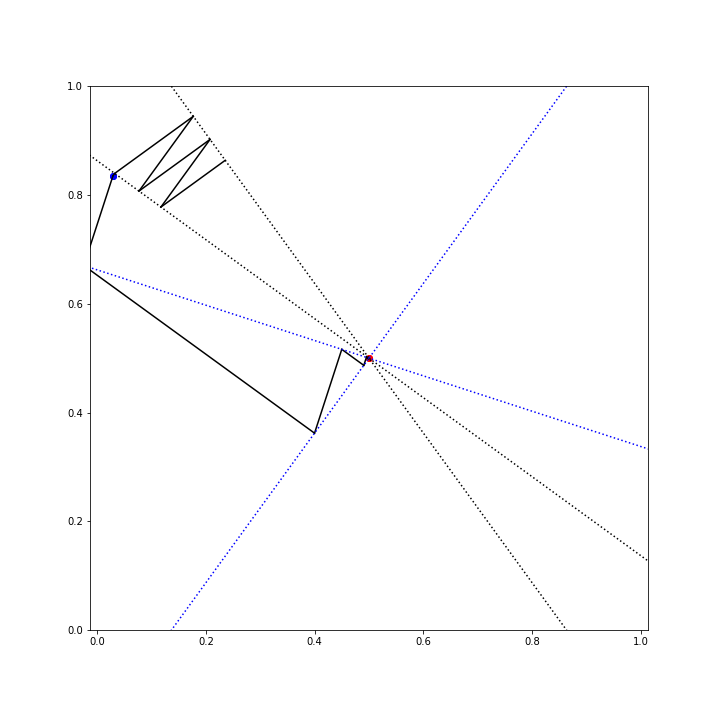
\includegraphics[width=0.475\linewidth]{examples/iterative/10D-firstepoch.png}
  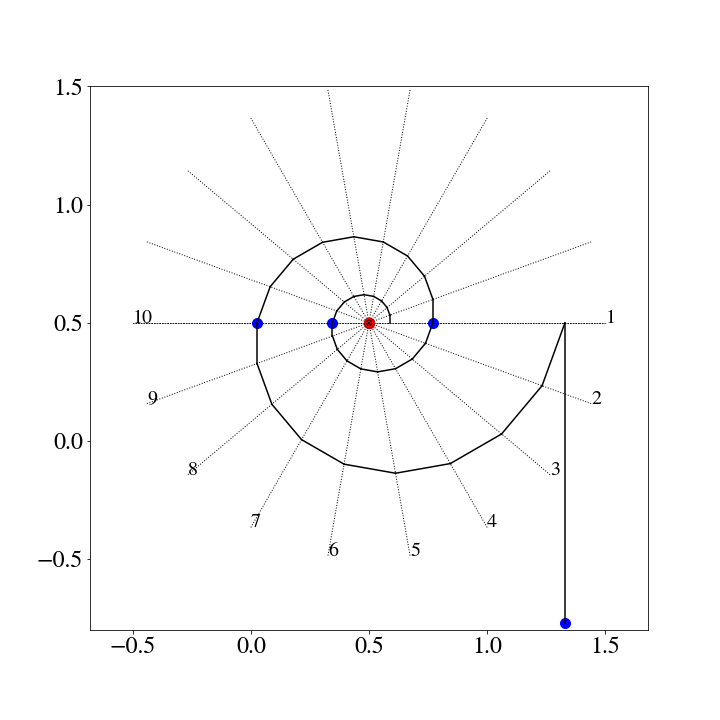
\includegraphics[width=0.475\linewidth]{examples/iterative/10D-fewepochs.png}

  \caption{
  Dotted lines show the solution contours for each row of the operator $A$.
  (Left): First epoch for iterating through 10 QoI.
  (Right): Three more epochs allows our estimate to get much closer to the true value.
  }
  \label{fig:iterative-linear-demo}
\end{figure}

The spiral shape is a result of the underlying geometry of this QoI map defined by rotations. The successive rows are so similar to each other that very little is ``learned'' between each iteration; the projection doesn't cover a large distance in $\pspace$.
At the end of these epochs, the estimate in the right panel of \ref{fig:iterative-linear-demo} is still far off from the true parameter value (the intersection of the contours).

To further underscore the lack of mutually distinct information in successive rows of the QoI, we choose two pairs of indices from among the ten available in order to define two QoI maps, the contours for which we plot in different colors in Fig.~\ref{fig:iterative-linear-demo-pair}.
We solve a total of ten 1-D inverse problems for each of them (five epochs) to match the budget of the previous example in the left panel of \ref{fig:iterative-linear-demo} (with ten maps and one epoch).

\begin{figure}
  \centering
  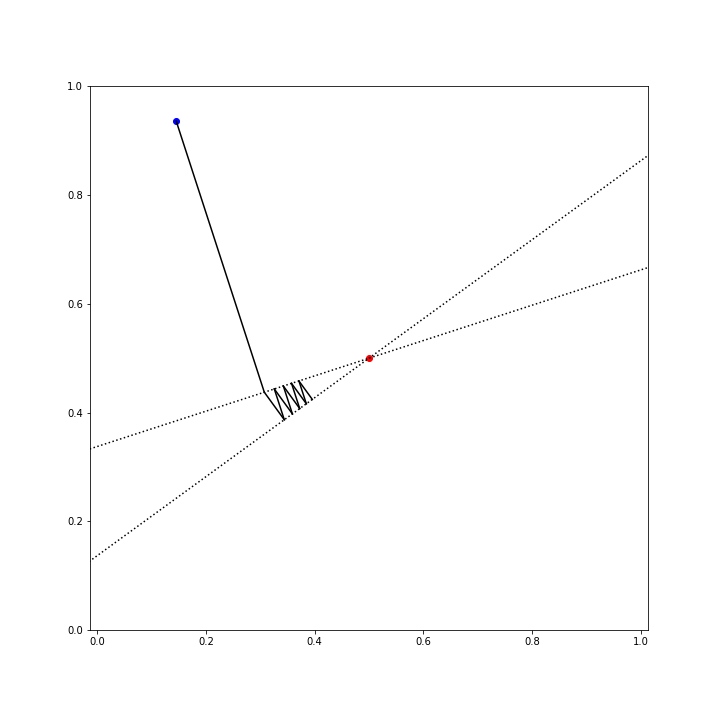
\includegraphics[width=0.475\linewidth]{examples/iterative/10D-fewepochs-pair.png}
  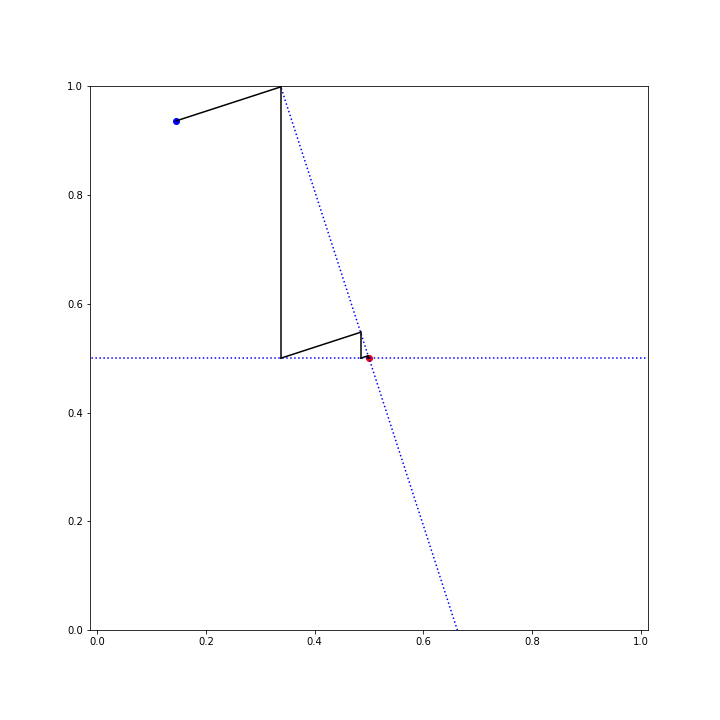
\includegraphics[width=0.475\linewidth]{examples/iterative/10D-fewepochs-pair-alt.png}
  \caption{
  Iterating through five epochs of two QoI, each formed by picking two of the ten available rows of $A$ at random.
  The random directions chosen on the left exhibit more redundancy than those on the right, so the same amount of iteration results in less accuracy.
  }
  \label{fig:iterative-linear-demo-pair}
\end{figure}

We observe that in Fig~\ref{fig:iterative-linear-demo-pair}, that there is much greater accuracy in estimating the true parameter value than in the case of Fig~\ref{fig:iterative-linear-demo}.
The reason for this difference is that there is more mutually distinct information between successive iterations of a pair of random rows of $A$ than there is between adjacent rows, as measured by the angle between the solution contours.

\subsection{Connection to Skewness}
If we are careful with how we construct maps or choose an iteration strategy, we can achieve considerably more accurate solutions with the same computational cost.
Had the choice of QoI components corresponded to a pair of rows that were orthogonal, the initial mean would converge to the reference value in a single epoch (two iterations), since there is no redundancy in information whatsoever.
This is equivalent to saying that we have an incentive to select rows that induce a QoI map with unit skewness.

\begin{figure}
  \centering
  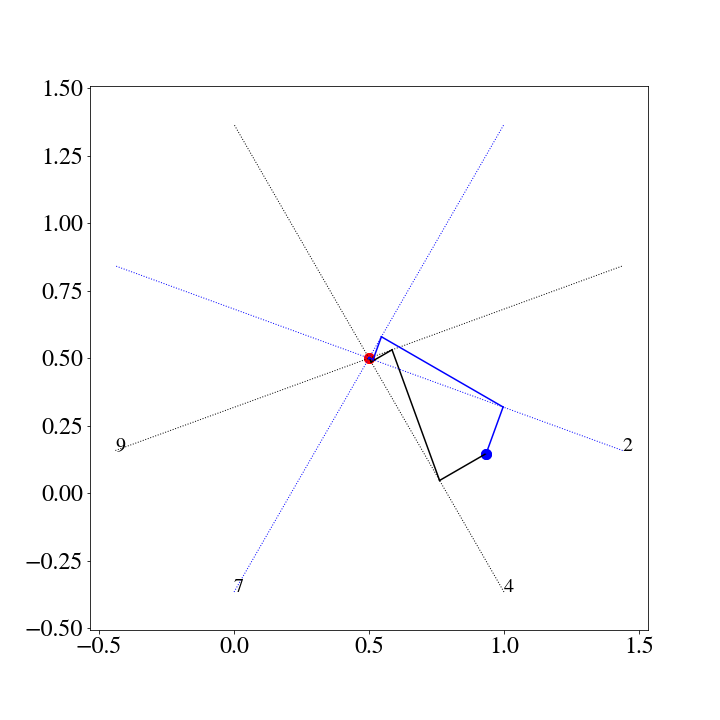
\includegraphics[width=0.475\linewidth]{examples/iterative/10D-firstepoch-pair-smart.png}
  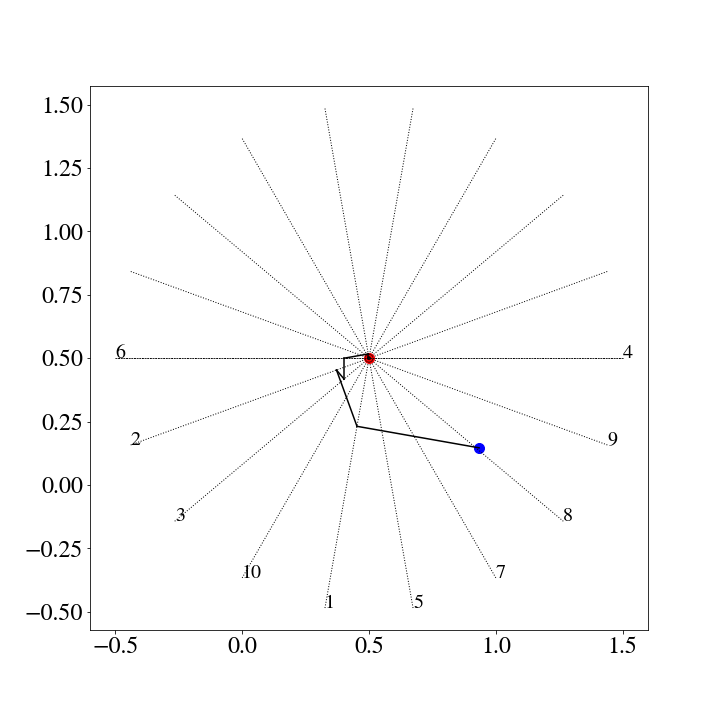
\includegraphics[width=0.475\linewidth]{examples/iterative/10D-firstepoch-rand.png}
  \caption{
  (Left): Iterating through a single epoch with a QoI formed by picking rows of $A$ which exhibit mutual orthogonality.
  (Right): Iterating through the rows of $A$ at a random order for a single epoch results in considerably more accuracy than doing so in the original order of rows of $A$.
  }
  \label{fig:iterative-linear-demo-smart}
\end{figure}


We show this in the left half of Figure~\ref{fig:iterative-linear-demo-smart} for two QoI maps with orthogonal pairs of components.
If instead no a priori analysis of the rows of $A$ and iteration through the available QoI at random is the chosen ordering, more accuracy is achieved with only ten iterations.
We show this in the right-half of Figure \ref{fig:iterative-linear-demo-smart}, which exhibits a more accurate estimate compared to \ref{fig:iterative-linear-demo} at the same computational cost.


\subsection{Comparisons and Convergence Results}
To make these results more concrete, we propose the following example:
We limit ourselves to solving 100 inverse problems (i.e. up to ten epochs for this map), with the \emph{only} difference between approaches being the order in which the rows of $A$ are used.
First, we use the QoI as they are presented: in order with respect to increased rotation angle (which defines the rows of $A$).
Next, we shuffle the rows of $A$ and then perform ten epochs using this permuted map.
Lastly, we create an ordering based on a random shuffling of ten sets of indices representing the rows of $A$.
The latter approach is similar to the second in that the same problems are solved the same number of times overall, but it lifts the restriction that a row must only be used once in each successive set of ten iterations (equal computational effort).

\begin{figure}
  \centering
  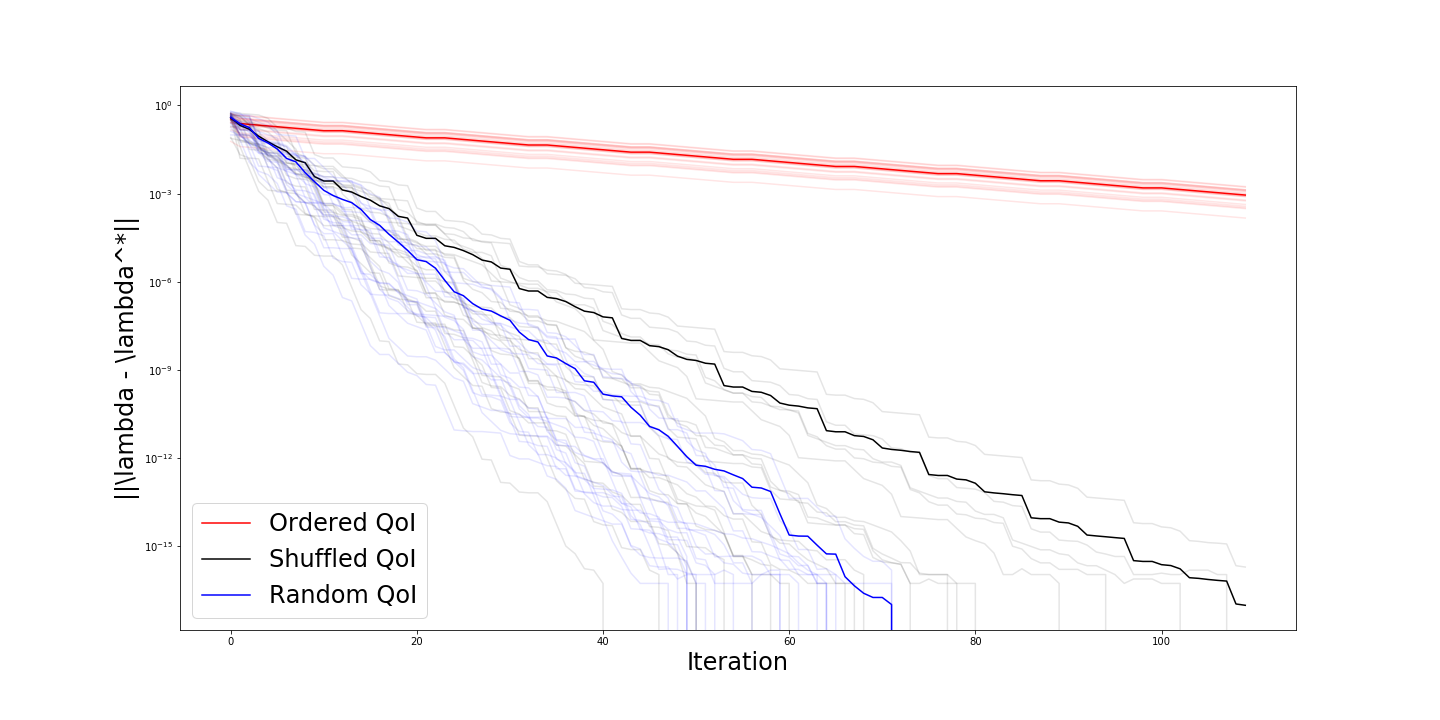
\includegraphics[width=0.95\linewidth]{examples/iterative/10D-convergence-comparison.png}
  \caption{
  Twenty different initial means are chosen and iterated on for three approaches.
  Individual experiments are transparent and the mean error is shown as solid lines.
  In the \emph{Ordered} approach, we iterate through the rows of $A$ as they are given to us for ten epochs.
  \emph{Shuffled QoI} refers to establishing a different random ordering of the rows of $A$ for each trial, and then
  using this ordering for ten epochs.
  Finally, in the \emph{Random QoI} approach, we choose a QoI at random for each of 100 iterations, where the ordering still ensures each row gets used ten times, representing the same overall set of inverse problems solved as the other two.
  }
  \label{fig:iterative-convergence-comparison}
\end{figure}

In Figure~\ref{fig:iterative-convergence-comparison}, it is shown that using the rows of $A$ sequentially performs very poorly (the error struggles to get past a single decimal place of accuracy), which aligns with ``spiraling'' seen in Figure~\ref{fig:iterative-linear-demo} where the first few epochs are plotted.
Shuffling the rows but requiring that every tenth iteration to use the same row (i.e., ensure same ordering for each epoch), leads to a considerable improvement by which sixteen decimal places of accuracy are achieved in under $100$ iterations.
In a few instances, the shuffled approach stumbles on an ordering that accelerates convergence, likely due to orthogonal pairs of rows in the shuffled order.
These cases exhibit the kind of behavior seen in the left panel of Fig~\ref{fig:iterative-linear-demo-smart}; in other words, sometimes random shuffling finds the ``smart'' rows to iterate through.
Since the ordering has no dependence on iteration number in the approach where we use random rows, we have more opportunities to find these successive orthogonal pairings, and so we see that on average, it takes fewer iterations to achieve the same accuracy.

%
% \subsection{Iterated Solutions for a PDE Example}\label{sec:iterated-nonlinear}
%
% Batch-updates is the connection to make here.
% We are going to set up the heatrod example here but place measurement devices throughout and record the measurements at several intervals in time, the point being here that the dimension of the QoI will be higher than the input space but it's okay because we're iterating.
%
% Some systems will be more informative early in time, others late, so the best thing to do is not really something we're going to answer, we're just going to show how this approach \emph{could} work in a situation like this where the data is streaming in over time.

\FloatBarrier
